\section{Resultados}
% Deben incluir los resultados de los experimentos, utilizando el formato mas
% adecuado para su presentacion. Deberan especicar claramente a que
% experiencia corresponde cada resultado. No se incluiran aqu corridas de
% maquina. Algo fundamental en su aprendizaje en la materia es la presentacion
% de resultados de forma clara y concisa para el lector

\subsection{Hipótesis}
Como vimos en la Introducción Teórica, Newton tiene convergencia cuadrática y Secante $supralineal$ (alrededor de 1.6).\\

Sería normal suponer que Newton tiene mejor performance dado que converge más rápido. Sin embargo para comparar performance, debemos considerar costo como rapidez de convergencia. Un algoritmo que converge rápido pero tarda algunos segundos por iteración podría tomar mas tiempo que uno que converge mas lento pero toma solo algunos milisegundos por iteración.\\

Podemos asumir que el costo de una iteración está marcado por la evaluación de la función, de hecho, este vendría a ser nuestro caso. Entonces la cantidad de evaluaciones de una función puede ser una buena medida de costo.\\

Secante solo requiere una evaluación de la función por iteración, dado que el valor de $f(x_{n - 1})$ se puede guardar de la iteración previa.\\

Newton requiere una evaluación de la función y otra de su derivada por iteración. Es complicado estimar el costo de evaluar la derivada en general. En algunos casos la derivada puede ser fácil de evaluar y en otros puede ser incluso mas difícil de evaluar que la función original.\\

Podemos asumir entonces, que en general, calcular la derivada es al menos tan costoso como calcular la función. Por lo tanto asumimos que Newton va a tomar dos evaluaciones por iteración.\\

Este análisis nos lleva a suponer que Secante debería ser mas performante que Newton en general.

\subsection{Casos de Prueba}
La aproximación inicial que tuvimos fue tomar cada uno de los parámetros, fijar los demás y hacer un análisis de cada uno de los factores de estudio (tiempo, iteraciones, convergencia, etc.) haciendo crecer los parámetros de turno. Claramente la cantidad de casos era mucha y en general los resultados eran difíciles de interpretar y no aportaban al propósito de develar si nuestra hipótesis se cumplía.\\

Por lo tanto decidimos que lo mejor sería solamente tomar un par de combinaciones de todas las posibles que nos parecieran que fueran representativas. A saber:\\

ACA PONER LOS CASOS PAPA!

\subsection{Gráficos}

Veamos algunos resultados graficamente:

\subsection{Cantidad de iteraciones f(x) con Newton y Secante}
Estos gráficos fueron generados con un inputs similares. En el caso de secante se utilizó el mismo $x_0$ y para $x_1 = 2x_0$. Podemos ver que ambos gráficos se comportan similarmente, a medida que el $x_0$ crece, crece la cantidad de iteraciones.\\

\begin{center}
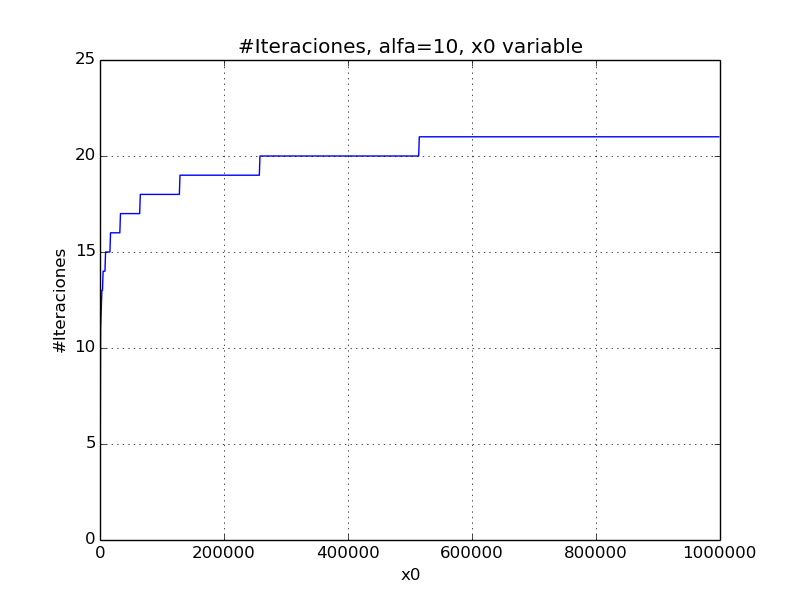
\includegraphics[scale=0.5]{graficos/iteraciones-f-newton-alfa_fijo-absoluto-0.001-alejando.png}\\
$f(x)$ aproximada con Newton, criterio de parada error absoluto igual a $0.001$
\end{center}

\begin{center}
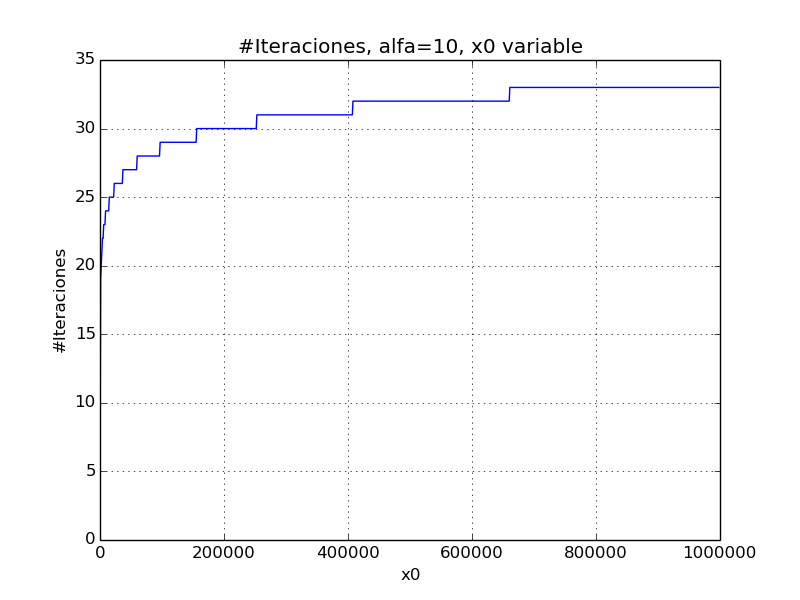
\includegraphics[scale=0.5]{graficos/iteraciones-f-secante-alfa_fijo-absoluto-0.001-alejando.png}\\
$f(x)$ aproximada con Secante, criterio de parada error absoluto igual a $0.001$
\end{center}

\subsection{Error Absoluto f(x) con Newton y Secante}
Al igual que en los gráficos anteriores acá también se realizaron las pruebas con inputs similares.\\

\begin{center}
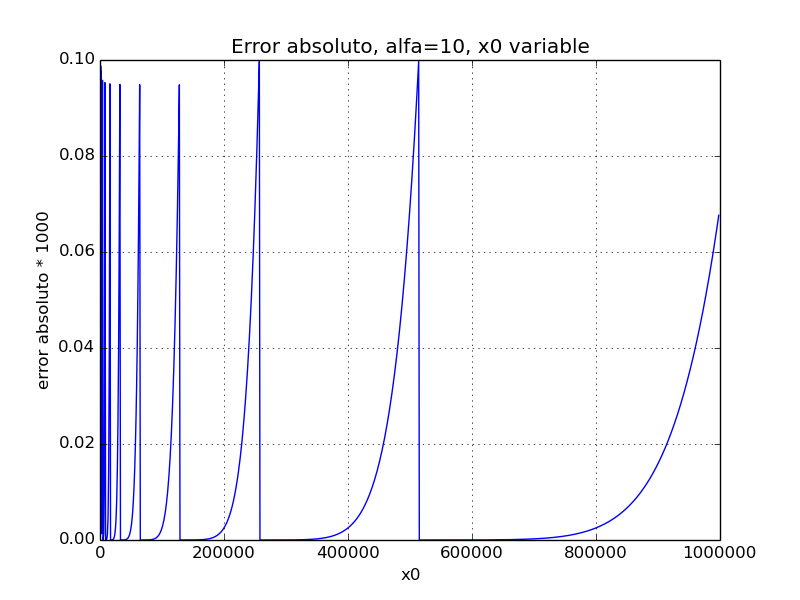
\includegraphics[scale=0.5]{graficos/x0s-f-newton-alfa_fijo-absoluto-0.001-alejando.png}\\
Newton. Criterio de parada: Error absoluto igual a 1 $\times$ $10^{-3}$
\end{center}

\begin{center}
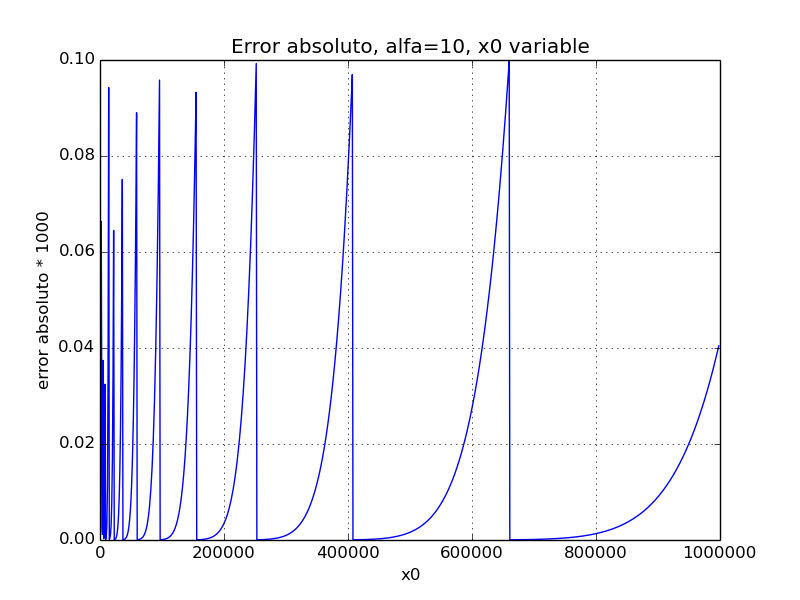
\includegraphics[scale=0.5]{graficos/x0s-f-secante-alfa_fijo-absoluto-0.001-alejando.png}\\
Secante. Criterio de parada: Error absoluto igual a 1 $\times$ $10^{-3}$
\end{center}


\subsection{Tiempo de Computo f(x) con Newton y Secante}
Nuevamente se utilizaron inputs similares para ambos gráficos. La idea era comparar los tiempos de CPU para cada método.\\

Las variaciones de tiempo se deben al hecho de que la máquina donde se realizan las pruebas corre tareas de fondo; quitando la mayoria de los procesos que corrían en la maquina y realizando las pruebas varias veces mostró que las variaciones de tiempo no siguen un patrón establecido.\\

A los valores de tiempo se les restó $0,03$ milisegundos, que se estima que es el tiempo fijo que el programa se toma en invocar la función \verb|gettimeofday()| dos veces (podemos ver que a veces, por cuestiones del scheduler de la CPU, las funciones toman dramáticamente menos tiempo en correr y hacer un cambio de contexto, por lo que el tiempo resulta "negativo" en unos pocos casos). Podemos observar luego que el tiempo para obtener los resultados incrementan en una curva logarítmica muy suave, correspondiente a la cantidad de iteraciones necesarias, no obstante la distancia de $x_0$ se tuvo que aumentar dramáticamente (hasta 1 millón) para que la diferencia sea claramente observable.\\

\begin{center}
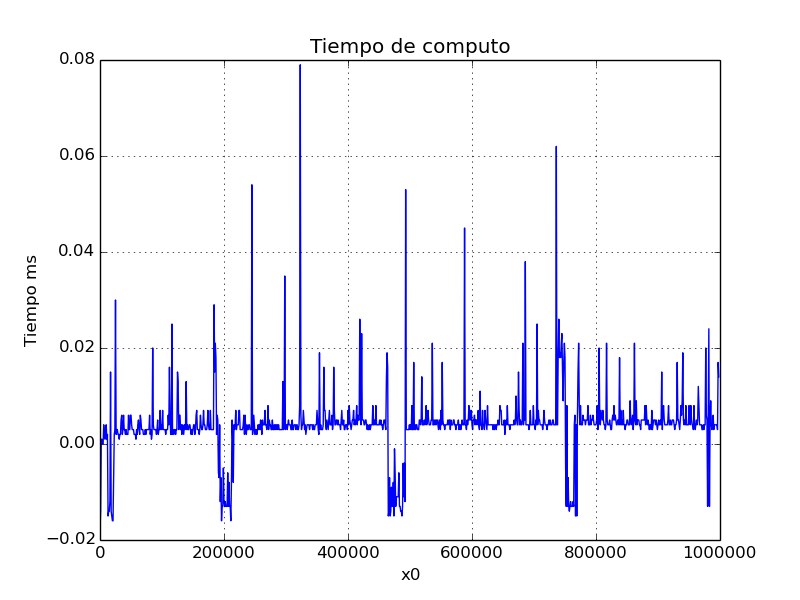
\includegraphics[scale=0.5]{graficos/tiempo-f-newton-alfa_fijo-absoluto-0.001-alejando.png}\\
Newton con $\alpha$ fijo y error absoluto de $0.001$ con $x_0$ creciente.
\end{center}

\begin{center}
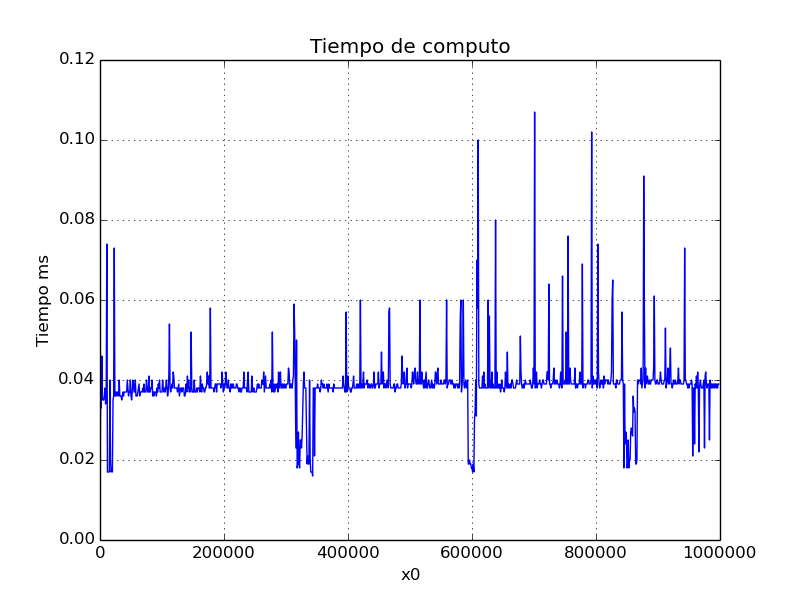
\includegraphics[scale=0.5]{graficos/tiempo-f-secante-alfa_fijo-absoluto-0.001-alejando.png}\\
Secante con $\alpha$ fijo y error absoluto de $0.001$ con $x_0$ creciente.
\end{center}

\subsection{Graficos para f(x) con error absoluto 0.0001}
Los siguiente gráficos detallan la resolución de $f(x)$ con Newton, específicamente cuando el $x_0$ inicial es cercano a la respuesta conocida, con $\alpha = 10$. Vemos que requiere una cantidad mucho menor de iteraciones, y el comportamiento del resultado es mucho más simple de entender.

\begin{center}
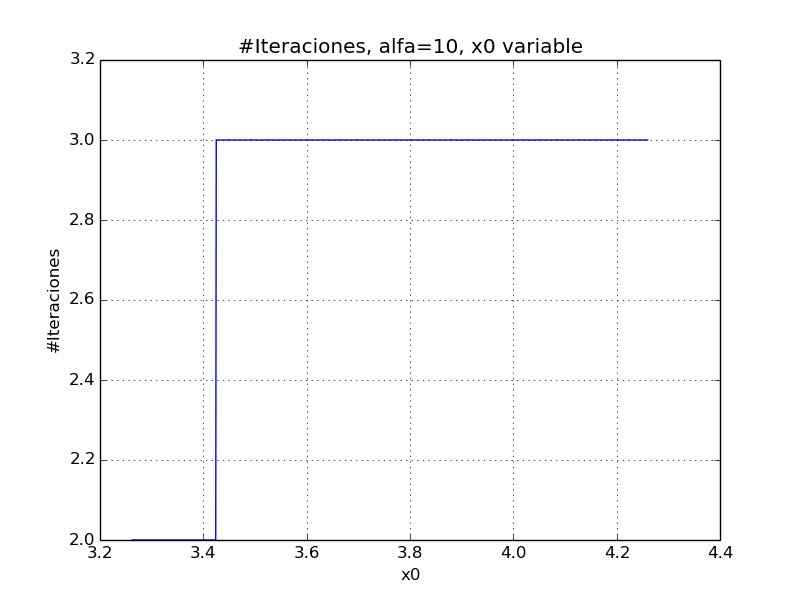
\includegraphics[scale=0.5]{graficos/iteraciones-f-newton-alfa_fijo-absoluto-0.0001-alejando_cercano.png}\\
Cantidad de iteraciones.
\end{center}

\begin{center}
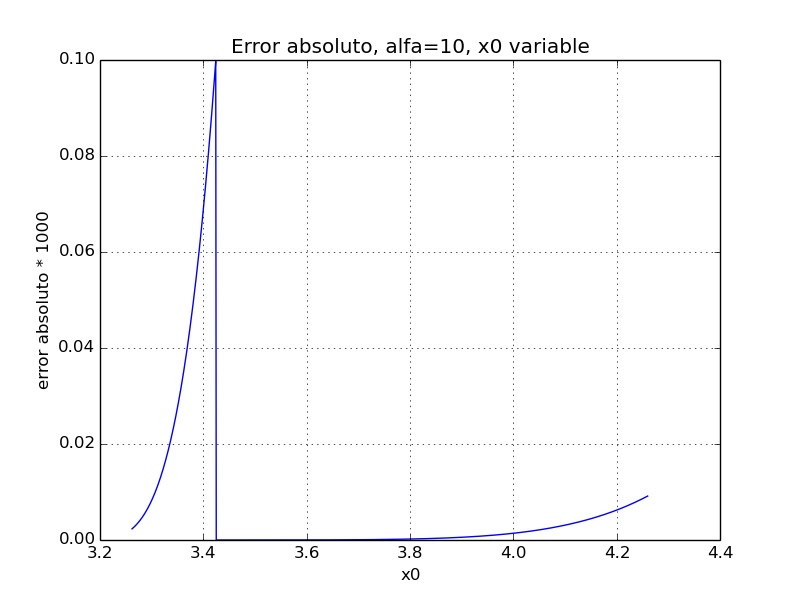
\includegraphics[scale=0.5]{graficos/x0s-f-newton-alfa_fijo-absoluto-0.0001-alejando_cercano.png}\\
Error absoluto.
\end{center}

\begin{center}
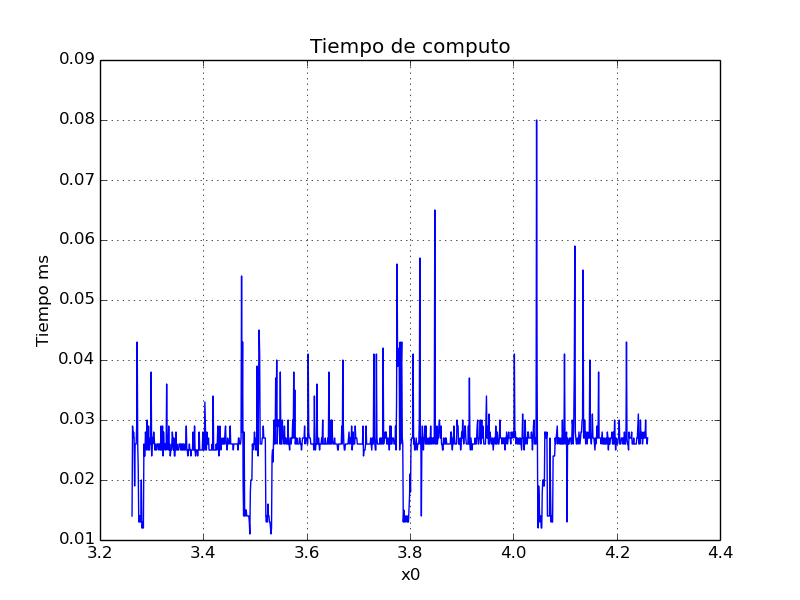
\includegraphics[scale=0.5]{graficos/tiempo-f-newton-alfa_fijo-absoluto-0.0001-alejando_cercano.png}\\
Tiempo de computo.
\end{center}

\subsection{Graficos para e(x)}

Los $x_0$ y $x_1$ se tomaron en $\frac{1}{\sqrt{\alpha}} + 0.001$ y superiores a $-\frac{1}{\sqrt{\alpha}} - 0.001$

Se observa que la función converge solo para un intervalo limitado, probablemente debido a que la función tiene dos asíntotas, y su derivada en los límites al infinito tiende a cero, dificultando cálculos por números demasiado grandes y demasiado chicos.

Se ve que el comportamiento es errático y difícil de predecir, en comparación a la resolución del inverso.

Las mismas observaciones sobre la dificultad de medir el tiempo de ejecución se aplican aquí.

\begin{center}
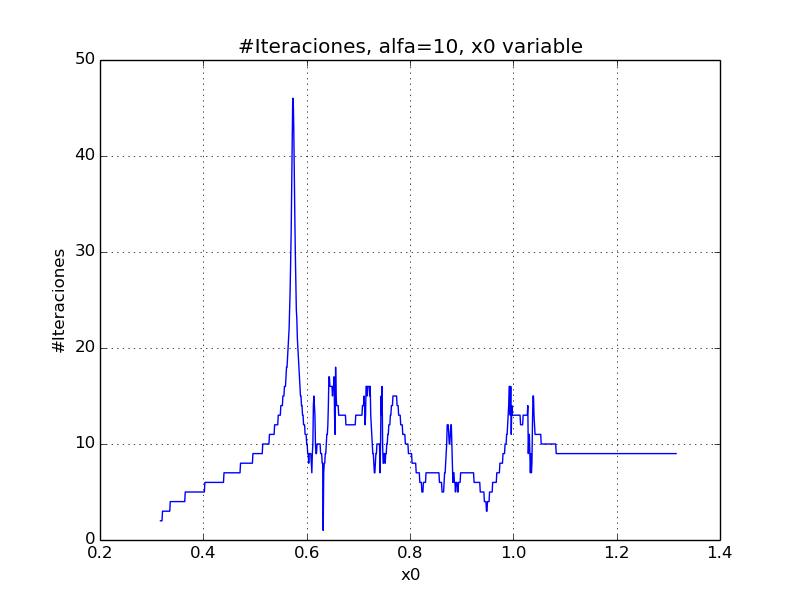
\includegraphics[scale=0.5]{graficos/iteraciones-e-secante-alfa_fijo-absoluto-0.0001-alejando.png}\\
poner titulos
\end{center}

\begin{center}
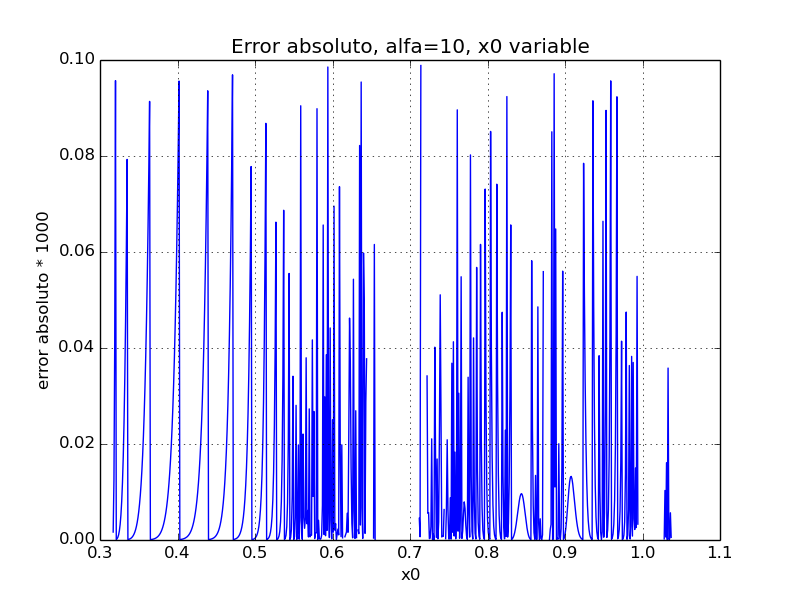
\includegraphics[scale=0.5]{graficos/x0s-e-secante-alfa_fijo-absoluto-0.0001-alejando.png}\\
poner titulos
\end{center}

\begin{center}
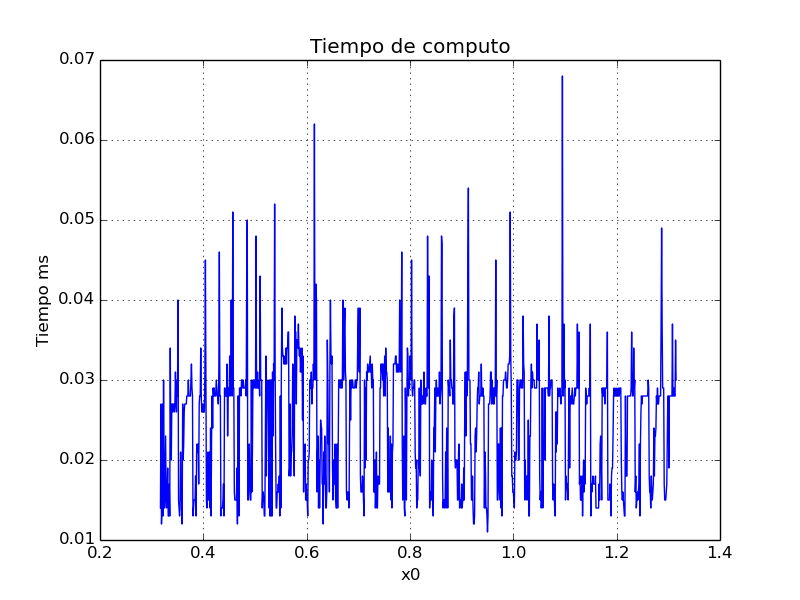
\includegraphics[scale=0.5]{graficos/tiempo-e-secante-alfa_fijo-absoluto-0.0001-alejando.png}\\
poner titulos
\end{center}

\begin{center}
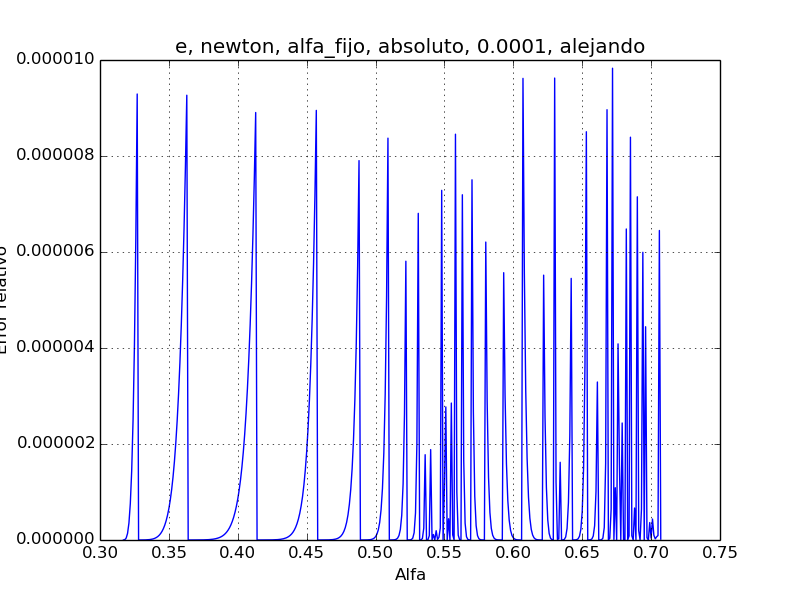
\includegraphics[scale=0.5]{graficos/relativo-e-newton-alfa_fijo-absoluto-0.0001-alejando.png}\\
poner titulos
\end{center}

\begin{center}
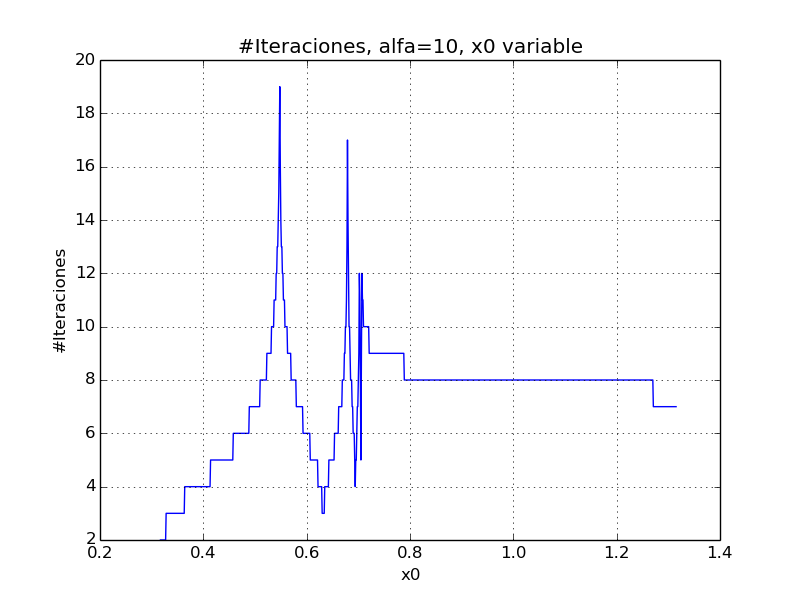
\includegraphics[scale=0.5]{graficos/iteraciones-e-newton-alfa_fijo-absoluto-0.0001-alejando.png}\\
poner titulos
\end{center}

\begin{center}
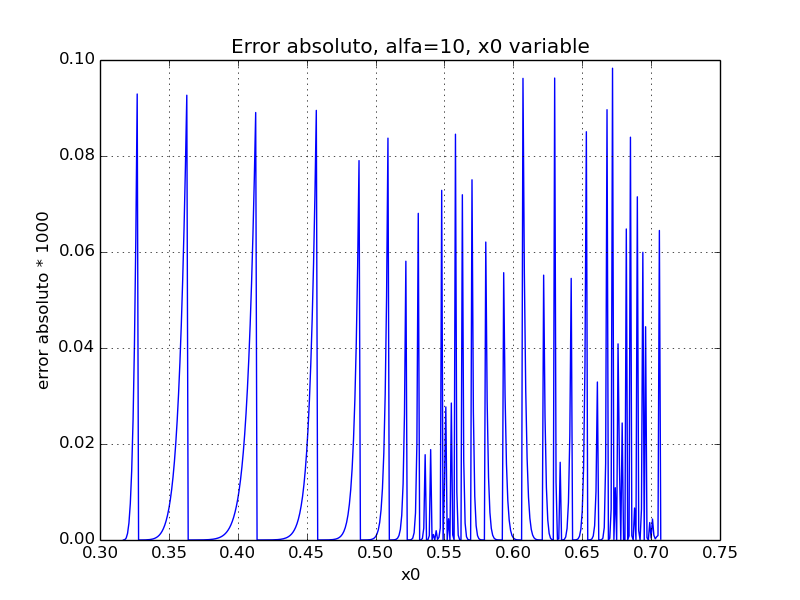
\includegraphics[scale=0.5]{graficos/x0s-e-newton-alfa_fijo-absoluto-0.0001-alejando.png}\\
poner titulos
\end{center}

\begin{center}
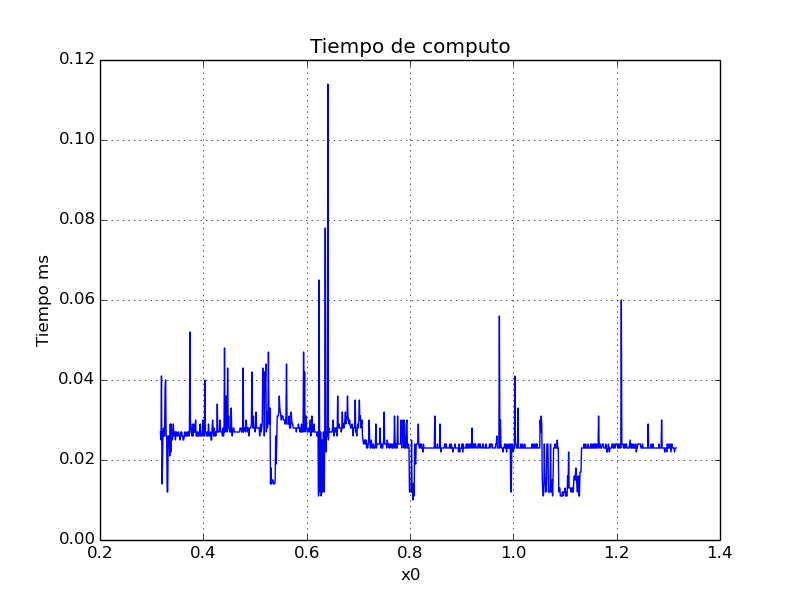
\includegraphics[scale=0.5]{graficos/tiempo-e-newton-alfa_fijo-absoluto-0.0001-alejando.png}\\
poner titulos
\end{center}

% Ver un grafico que muestra los picos del error relativo conforme el alapha se aleja del x0. La explicacion es que conforme mas lejos esta el x0 del resultado, tiene que realizar mas itreraciones y el error relativo de la ultima iteracion que vale crece conforme aumenta la distancia entre alpah y x0 hasta que la iteracion no califica para entrar en el criterio de tension relativo. Entonces debe realizar una iteracion mas que resulta mas precisa y asi sucesivamente

% Hay que un hacer un grafico del mismo experimento pero con el numero de iteraciones y queremos mosrtar que conforme la distancaio del x0 al alpha crece pasa que la cant de iteraciones para converger aumenta.

% Hacer un exp de un alpha fijo con un x0 que se va corriendo. Para observar las iteraciones sobre un valor fijo con la distancia entre x0 y alpha, corriendo el x0. Ademas un grafico de tiempo.

% Un grafico de newton de 1 al 10000 con error absoluto con x0 cercanos al resultado real y compararlo con las iteraciones del relativo

%Los tipos de experimentos:
%* Comparar newton y secante para f(x) y e(x) en función de:
%    1. cantidad de iteraciones
%    2. tiempo de ejecución
%    3. error relativo, error absoluto
%    4. orden de convergencia
%* Los tipos de inputs a utilizar pueden ser:
%    1. crecientes de 1 a 1000 en intervalos de 1, 5 y 10
%    2. crecientes de 0 a 1 en intervalos chiquitos, la idea es ver cuando forzamos a que la precisión se pierda
%    2. aleatorios con magnitud definida